\documentclass[12pt,]{article}
\usepackage{lmodern}
\usepackage{amssymb,amsmath}
\usepackage{ifxetex,ifluatex}
\usepackage{fixltx2e} % provides \textsubscript
\ifnum 0\ifxetex 1\fi\ifluatex 1\fi=0 % if pdftex
  \usepackage[T1]{fontenc}
  \usepackage[utf8]{inputenc}
\else % if luatex or xelatex
  \ifxetex
    \usepackage{mathspec}
    \usepackage{xltxtra,xunicode}
  \else
    \usepackage{fontspec}
  \fi
  \defaultfontfeatures{Mapping=tex-text,Scale=MatchLowercase}
  \newcommand{\euro}{€}
\fi
% use upquote if available, for straight quotes in verbatim environments
\IfFileExists{upquote.sty}{\usepackage{upquote}}{}
% use microtype if available
\IfFileExists{microtype.sty}{%
\usepackage{microtype}
\UseMicrotypeSet[protrusion]{basicmath} % disable protrusion for tt fonts
}{}
\usepackage[margin=1in]{geometry}
\ifxetex
  \usepackage[setpagesize=false, % page size defined by xetex
              unicode=false, % unicode breaks when used with xetex
              xetex]{hyperref}
\else
  \usepackage[unicode=true]{hyperref}
\fi
\hypersetup{breaklinks=true,
            bookmarks=true,
            pdfauthor={},
            pdftitle={},
            colorlinks=true,
            citecolor=blue,
            urlcolor=black,
            linkcolor=black,
            pdfborder={0 0 0}}
\urlstyle{same}  % don't use monospace font for urls
\setlength{\parindent}{0pt}
\setlength{\parskip}{6pt plus 2pt minus 1pt}
\setlength{\emergencystretch}{3em}  % prevent overfull lines
\setcounter{secnumdepth}{0}

%%% Use protect on footnotes to avoid problems with footnotes in titles
\let\rmarkdownfootnote\footnote%
\def\footnote{\protect\rmarkdownfootnote}

%%% Change title format to be more compact
\usepackage{titling}

% Create subtitle command for use in maketitle
\newcommand{\subtitle}[1]{
  \posttitle{
    \begin{center}\large#1\end{center}
    }
}

\setlength{\droptitle}{-2em}
  \title{}
  \pretitle{\vspace{\droptitle}}
  \posttitle{}
  \author{}
  \preauthor{}\postauthor{}
  \date{}
  \predate{}\postdate{}

\usepackage{lineno}
\linenumbers
\usepackage{setspace}
\doublespacing
\usepackage[document]{ragged2e}
\usepackage{color, soul}
\usepackage{graphicx}


\begin{document}

\maketitle


\renewcommand*{\thefootnote}{\fnsymbol{footnote}}

\begin{centering}
\textbf{\large{Forecasting climate change impacts on plant populations over large spatial extents}}

\textsc{\small{Andrew T. Tredennick\footnote{Corresponding author: atredenn@gmail.com}\textsuperscript{1}, Mevin B. Hooten\textsuperscript{2,3,4}, Cameron L. Aldridge\textsuperscript{5}, Collin G. Homer\textsuperscript{6}, Andrew R. Kleinhesselink\textsuperscript{1}, and Peter B. Adler\textsuperscript{1}}}

\textit{\small{\textsuperscript{1}Department of Wildland Resources and the Ecology Center, 5230 Old Main Hill, Utah State University, Logan, Utah 84322 USA}} \\
\textit{\small{\textsuperscript{2}U.S. Geological Survey, Colorado Cooperative Fish and Wildlife Research Unit, Colorado State University, Fort Collins, CO 80523 USA}} \\
\textit{\small{\textsuperscript{3}Department of Fish, Wildlife, and Conservation Biology, Colorado State University, Fort Collins, CO 80523 USA}} \\
\textit{\small{\textsuperscript{4}Department of Statistics, Colorado State University, Fort Collins, CO 80523 USA}} \\
\textit{\small{\textsuperscript{5}Natural Resource Ecology Laboratory and Department of Ecosystem Science and Sustainability, Colorado State University, Fort Collins, CO, in cooperation with US Geological Survey, Fort Collins Science Center, Fort Collins, CO}}\\
\textit{\small{\textsuperscript{6}U.S. Geological Survey (USGS) Earth Resources Observation and Science (EROS) Center, Sioux Falls, SD 57198 USA}}

\end{centering}

\renewcommand*{\thefootnote}{\arabic{footnote}}

\setcounter{footnote}{0}

\subsection{Abstract}\label{abstract}

Plant population models are powerful tools for predicting climate change
impacts in one location, but are difficult to apply at landscape scales.
We overcome this limitation by taking advantage of two recent advances:
remotely-sensed, species-specific estimates of plant cover and
statistical models developed for spatio-temporal dynamics of animal
populations. Using computationally efficient model reparameterizations,
we fit a spatiotemporal population model to a 28 year time series of
sagebrush (\emph{Artemisia} spp.) percent cover over a \(2.5\times5\) km
landscape in southwestern Wyoming while formally accounting for spatial
autocorrelation. We include interannual variation in precipitation and
temperature as covariates in the model to investigate how climate
affects the cover of sagebrush. We then use the model to forecast the
future abundance of sagebrush at the landscape scale under projected
climate change, generating spatially explicit estimates of
\textcolor{blue}{sagebrush population trajectories} that have, until
now, been impossible to produce at this scale. Our broad-scale and
long-term predictions are rooted in small-scale and short-term
population dynamics and provide an alternative to predictions offered by
species distribution models that do not include population dynamics. Our
approach,
\textcolor{blue}{which combines several existing techniques in a novel way, demonstrates the use of}
remote sensing data to model population responses to environmental
change that play out at spatial scales far greater than the traditional
field study plot.

\emph{Key words: population model, climate change, forecasting,
spatiotemporal model, remote sensing, sagebrush}, Artemisia,
\emph{dimension reduction}

\subsection{Introduction}\label{introduction}

Forecasting the impacts of climate change on plant populations and
communities is a central challenge for ecology (Clark et al. 2001,
Petchey et al. 2015). Population models are ideally suited for meeting
such a challenge because they provide a way to link climate drivers
directly to population dynamics (Hare et al. 2010, Adler et al. 2012,
Ross et al. 2015, Shriver 2015). However, inference from population
models is typically limited to small spatial extents because the data
required is difficult to collect across broad species ranges. Almost
every study of plant population dynamics relies on demographic
observations recorded at the meter to sub-meter scale (see, e.g.,
Salguero-G{ó}mez et al. 2015). Local-scale demographic data make
building population projection models an easy task (Ellner and Rees
2006, Rees and Ellner 2009, Adler et al. 2012), but it is very difficult
to extrapolate small-scale studies to large spatial extents with any
certainty because the data likely only represent a small subset of
parameter space and environmental conditions (Freckleton et al. 2011,
Queenborough et al. 2011). The real challenge is not to simply make
population forecasts, but to do so at spatial scales relevant to policy
and management decisions (Queenborough et al. 2011).

The ideal tool would be a \textcolor{blue}{broad}-scale, dynamic
population model (Schurr et al. 2012, Merow et al. 2014), but developing
useful models at this scale has been limited by the availability of time
series data at large spatial extents and statistical methods for fitting
high-dimensional spatial models. Fortunately, new advances in remote
sensing and statistics now allow us to overcome both of these
limitations. First, new remote-sensing (RS) methods are now producing
accurate time series of species-specific plant cover at landscape
scales. These data can be fit with dynamic population models which
include yearly fluctuations in climate as covariates. Such RS time
series have revolutionized models of how climate affects ecosystem-level
processes (e.g., Running et al. 2004) and have been used to detect
long-term trends in plant population abundance (e.g., Homer et al.
2015), but they have yet to be used to drive a dynamic population model.
Second, animal population modelers have developed dimension reduction
and reparameterization techniques to efficiently fit high-dimension
spatiotemporal models (see Conn et al. 2015 for a review). These new
statistical methods have yet to be applied to RS-derived plant
population data at broad scales.

Large-scale, spatially-explicit population models based on RS data could
offer a valuable new way to investigate the effects of large-scale
environmental changes playing out at landscape and regional scales. Most
current assesments of how plant and animal populations will respond to
climate change rely on species distribution models (SDMs). SDMs rely on
static associations between contemporary climate and a species'
distribution or, more rarely, abundance to project future distribution
or abundance (Elith and Leathwick 2009) and they are easily applied at
landscape to continental scales (e.g., Maiorano et al. 2013, Clark et
al. 2014). However, the short-term and small-scale population dynamics
that actually drive the large-scale distributions of species are not
represented in most SDMs. Because SDMs typically rely on occurence data,
their projections of habitat suitability or probability of occurence
provide little information on the future states of populations in the
core of their range -- areas where a species exists now and is expected
to persist in the future (Ehrl{é}n and Morris 2015). Furthermore,
because they lack short-term dynamics, SDMs usually cannot produce any
estimate of the rate at which local populations will increase or
decrease in the near-term and instead project a future equilibrium
species distribution that may or may not ever be reached. Direct
validation of such predictions is extremely rare (Roberts and Hamann
2012). Large-scale dynamic population models could overcome these
limitations. They would produce spatially-explicit estimates of species
abundance within the species range (Ehrl{é}n and Morris 2015), have the
potential to model expansion in abundance outside the range when coupled
with dynamic models of dispersal, and would provide testable predictions
of how populations should respond to short-term climate perturbations.
These short-term predictions also would give modelers the opportunity to
repeatedly validate and refine their models (Luo et al. 2011).

Sagebrush (\emph{Artemisia} spp.) ecosystems offer an ideal testing
ground for new spatially explicit population models derived from RS
data. Sagebrush species are widely distributed (Kuchler 1964), they are
sensitive to climate (Perfors et al. 2003, Miglia et al. 2005, Poore et
al. 2009, Dalgleish et al. 2011, Xian et al. 2012, Apodaca 2013,
Schlaepfer et al. 2014a, 2014b, Harte et al. 2015, Homer et al. 2015),
new landscape and regional scale time series of sagebrush cover are now
being produced from aerial imagery (Homer et al. 2012), and forecasts of
future sagebrush ecosystems are in high demand due to the precarious
conservation status of the greater sage-grouse (\emph{Centrocercus
urophasianus}) (Arnett and Riley 2015). SDMs typically predict that much
of the area occupied by sagebrush ecosystems today will become
unsuitable for sagebrush due to climate change, resulting in a dramatic
loss in the extent of sagebrush habitat by the end of this century
(Shafer et al. 2001, Neilson et al. 2005, Bradley 2010, Schlaepfer et
al. 2012, Still and Richardson 2015). Ecohydrology models supply a
possible mechanism for sagebrush losses predicted by SDMs: climate
warming could lead to earlier snowmelt, increased evaporation and
ultimately less recharge of deeper soil layers in the spring (Schlaepfer
et al. 2012, 2014a). In warmer parts of its range, increased temperature
could be especially detrimental to sagebrush as it depends on water from
deeper soil to survive and grow in this arid region (Pechanec et al.
1937, Schlaepfer et al. 2011, Germino and Reinhardt 2014). In contrast,
at higher elevations and in colder regions, warming and earlier snowmelt
could lengthen the growing season and increase sagebrush occurrence
(Schlaepfer et al. 2012, 2014a). Direct observations of individual
plants and experimental plots tend to agree with these models: growth
tends to respond negatively to spring and summer temperatures (Miglia et
al. 2005, Poore et al. 2009, Apodaca 2013) except at higher elevations
where earlier snowmelt may allow for a longer growing season (Perfors et
al. 2003, Harte et al. 2015). A large-scale, spatially-explicit
population model for sagebrush driven by interannual climate variability
would provide a valuable new tool for assessing how sagebrush could
respond to climate change in the future.

Building on recent technological advances in spatial statistics (Latimer
et al. 2009, Conn et al. 2015) and anticipating ever-increasing
availability of RS data (He et al. 2015), we demonstrate how large-scale
plant population models could be used to predict population impacts of
climate change. \textcolor{blue}{As a proof-of-concept, we use} a
process model motivated by Gompertz density-dependent population growth
and a remotely-sensed time series of sagebrush cover from Wyoming (Homer
et al. 2012, 2015). We account for spatial autocorrelation with
dimension reduction techniques (Latimer et al. 2009, Conn et al. 2015)
and produce spatially-explicit estimates of sagebrush percent cover.
\textcolor{blue}{Unlike most SDMs, our approach models the dynamics of plant abundance through time, and thus, is a population model, in the same spirit that models of animal counts through time are population models.}
The modeling framework we propose can be applied to any
spatially-explicit time series of plant cover or density, but its
application to remotely-sensed data products offers the greatest
potential to combine the information of population models (e.g.,
population status \textcolor{blue}{and temporal dynamics}) and the
spatial extent of species distribution models.

\subsection{Materials and Methods}\label{materials-and-methods}

\subsubsection{Data}\label{data}

\paragraph{Remotely-sensed time
series}\label{remotely-sensed-time-series}

To demonstrate our modeling approach, we use a subset of a
remotely-sensed time series of sagebrush (\emph{Artemisia} spp.) canopy
cover in Wyoming (Homer et al. 2012). As part of a separate study,
\textcolor{blue}{Homer et al. 2012 estimated} sagebrush percent cover
using a regression tree to relate ground reflectances retrieved by three
sources of optical imagery (QuickBird, Landsat, and AWiFS) to 1,780
field observations of sagebrush cover distributed across Wyoming. The
regression tree model was further validated using another 297 field
observations. For Wyoming sagebrush, the model achieved an \(R^{2}\) =
0.65 and an out-of-sample RMSE of 5.46\% (Homer et al. 2012). To
hind-cast sagebrush cover the regression tree model was applied to
historical remote sensing images
\textcolor{blue}{to generate yearly predictions of sagebrush cover for all of Wyoming for the years 1984-2011}.
This resulted in an annual time series of sagebrush cover at 30 meter
resolution from 1984 to 2011 (Fig. B1). In this
\textcolor{blue}{remote sensing product}, values represent the
percentage of a 30 \(\times\) 30 meter pixel covered by sagebrush. In
our study, we focused on a 5,070 \(\times\) 2,430 meter subset totaling
13,689 30 \(\times\) 30 meter pixels each year (Fig. 1). Thus, the
subset of the \textcolor{blue}{remote sensing product} we use contains
369,603 observations spanning 27 year-to-year transitions (27 years
\(\times\) 13,689 pixels).

\paragraph{Climate covariates}\label{climate-covariates}

Our approach models interannual changes in plant cover as a function of
seasonal climate variables. We used daily historic weather data for the
center of our study site from the NASA Daymet data set (\emph{available
online})\footnote{\url{http://daymet.ornl.gov/}}. The Daymet weather
data are interpolated between coarse observation units and capture some
spatial variation. We relied on weather data for the centroid of our
study area. We calculated five climate variables from the Daymet data
for the time period coinciding with our remotely sensed data (1984 to
2011).

We narrowed our focus to climate covariates we know are important for
sagebrush and that could be calculated from general circulation model
projections. The five climate variables in our population model are: (1)
cumulative, ``water year'' precipitation for year \emph{t}-2
(\emph{lagPpt}), (2) year \emph{t}-1 fall through summer precipitation
(\emph{ppt1}), (3) year \emph{t} fall through summer precipitation
(\emph{ppt2}), (4) year \emph{t}-1 average spring temperature
(\emph{TmeanSpr1}), and (5) year \emph{t} average spring temperature
(\emph{TmeanSpr2}), where \emph{t-1} to \emph{t} is the transition of
interest. We selected these variables \emph{a priori} based on previous
studies (see \emph{Introduction}), though not all emerge as important
predictors in our model.

\subsubsection{Additive spatio-temporal model for sagebrush
cover}\label{additive-spatio-temporal-model-for-sagebrush-cover}

We use a descriptive model for sagebrush cover that includes additive
spatial and temporal effects similar to that described by Conn et al.
(2015). Interannual change in percent cover represents the integrated
outcome of recruitment, survival, growth, and retrogression (shrinkage)
of individual plants from year to year. We model observed integer
percent cover (\emph{y}) in cell \emph{i} at time \emph{t} as
conditionally Poisson

\vspace{-4em}\begin{align}
y_{i,t} \sim \text{Poisson}(\mu_{i,t}),
\end{align}\vspace{-4em}

where \(\mu_{i,t}\) is the expected percent cover of pixel \emph{i} in
year \emph{t}

\vspace{-4em}\begin{align}
\text{log}(\mu_{i,t}) &= \underbrace{\beta_{0,t} + \beta_{1}y_{i,t-1}}_\text{temporal + dens. dep} + \underbrace{\textbf{x}_{t}'\boldsymbol{\gamma}}_\text{climate} + \underbrace{\eta_{i}}_\text{spatial}.
\end{align}\vspace{-3em}

Our model of percent cover change includes a density-dependent effect of
log-transformed cover in the previous year (\(y_{i,t-1}\)), climate
effects (\(\textbf{x}_t\)), and a spatial random effect (\(\eta\)) for
each pixel \emph{i}. Climate effects were standardized
{[}\((x_{i}-\bar{x}) / \sigma(x)\){]} to improve convergence during the
model fitting stage and to allow for easier prior specification. The
intercept, \(\beta_{0,t}\), was allowed to vary through time; these
random year effects recognize that all observations from a particular
year share the same climate covariates and thus are not independent. We
used a Poisson likelihood because integer percent cover values in the
sagebrush data product can be considered a form of count data. We also
evaluated a negative binomial model, but found little evidence for
overdispersion beyond what our model was already accomodating via the
spatial random effects (\(\boldsymbol{\eta}\)). There was no evidence of
zero-inflation in our data, but see below (\emph{Accomodating zeros})
for how we handled the small number of zero percent cover observations.
\textcolor{blue}{We assume that the remotely sensed estimates of percent cover are "true" and free of error.}
\textcolor{blue}{This need not be the case, and if measurement or sampling error is known then it could be included in our Bayesian model as a "sampling model"}
(Hobbs and Hooten 2015).

The spatial random effect (\(\boldsymbol{\eta}\)) accounts for spatial
autocorrelation among pixels that occur near each other in space. Thus,
\(\boldsymbol{\eta}\) acts as an offset on the intercept
(\(\beta_{0,t}\)), creating a spatial field that defines how pixels
differ from the mean, on average, in space (e.g., areas of perennially
low or high cover, relative to average cover). Fitting the model with a
spatial random effect (\(\eta\)) is computationally demanding for large
data sets like ours. The computational demand is due to the required
calculations of the spatial covariance matrices, which increase as a
cubic function of the number of locations (Wikle 2010). Key to our
approach is a dimension reduction strategy that greatly reduces the
number of parameters needed to be estimated to account for spatial
variation by reducing the size of the spatial covariance matrices that
need to be inverted at each MCMC iteration. Fitting models that
appropriately account for spatial autocorrelation over large spatial
extents would not be feasible without these modern techniques. Our
dimension reduction strategy expresses the high dimensional spatial
random effect, \(\boldsymbol{\eta}\), as the product of an expansion
matrix, \textbf{K}, and a smaller parameter vector,
\(\boldsymbol{\alpha}\) (e.g., Hooten et al. 2003, Hooten and Wikle
2007, Conn et al. 2015). We can then approximate the spatial effect as

\vspace{-4em}\begin{align}
\boldsymbol{\eta} &\approx \textbf{K}\boldsymbol{\alpha}, \\
\alpha_{m} &\sim \text{Normal}(0,\sigma_{\eta}^2).
\end{align}\vspace{-4em}

In this case, \(\boldsymbol{\alpha}\) is a \(m \times 1\) vector of
reduced spatial random effects, and \textbf{K} is a \(S \times m\)
matrix that maps the reduced effects to the full \emph{S}-dimensional
space, where \emph{S} is the total number of observed locations. Thus,
we are able to reduce the effective number of parameters from \({S}\) to
\(m\).

The last remaining obstacle is to parameterize the matrix of basis
functions, \textbf{K}. We use kernel convolution (Barry and Hoef 1996,
Higdon 1998) to interpolate the spatial random effect between \emph{m}
``knots'' that are nonrandomly distributed across the space of our study
area. This means we are modeling spatial random effects at the knot
level, and we use \textbf{K} to interpolate those effects between knots.
We use an exponential kernel density to define the distance-decay
function around the knots (\textbf{w}), such that the entries of
\textbf{K} are

\vspace{-4em}\begin{align}
K_{s,m} &= w_{s,m} / \sum_{s=1}^{S} w_{s,m}
\end{align}\vspace{-4em}

where

\vspace{-4em}\begin{align}
w_{s,m} &= \text{exp}\left(\frac{-d_{s,m}}{\sigma}\right)
\end{align}\vspace{-4em}

and \(d_{s,m}\) is the Euclidean distance between the centroid of sample
cell \emph{s} and the location of knot \emph{m}, and \(\sigma\) is the
kernel bandwidth. It is possible, through exhaustive model selection and
fitting, to determine the optimal form of the kernel and to estimate
optimal values for \(\sigma\) (Higdon 2002, Hooten and Hobbs 2015).
However, given the relative size of our dataset and computational
limitations, we defined kernels around 231 knots (Fig. C2) whose nearest
neighbor distances are approximately equal to the range of spatial
dependence in residuals from a simple GLM fit without climate covariates
and the spatial random effect (\textasciitilde{}500 meters; Appendix C).
An infinite number of knots would result in an exact representation of
the spatial process and covariance model. Computationally, using an
infinite number of knots is not possible, thus the use of dimension
reduction techniques serves as an approximation, where the accuracy
increases with the number of knots. Given the tradeoff between knot
number and computation time, we chose to base our knot number on the
spatial dependence as described above.

The Bayesian posterior distribution of our spatio-temporal model can be
expressed as

\vspace{-4em}\begin{align}
[\boldsymbol{\beta}, \boldsymbol{\gamma}, \boldsymbol{\alpha}, \sigma_{\eta}^2 | \textbf{y}] &\propto \left( \prod_{t=1}^{T} \prod_{i=1}^{n} [y_{i,t} | \beta_{0,t}, \beta_{1}, \boldsymbol{\gamma},\boldsymbol{\alpha}] [\beta_{0,t}|\bar{\beta_{0}}, \sigma_{\beta_{0}}^2] \right) \times \\
&\left(\prod_{m=1}^{M}[\alpha_m|\sigma_{\eta}^2]\right)[\bar{\beta_{0}}][\beta_{1}][\boldsymbol{\gamma}][\sigma_{\beta_{0}}^2][\sigma_{\eta}^2]. \nonumber
\end{align}\vspace{-4em}

\subsubsection{Accomodating zeros}\label{accomodating-zeros}

Our process model (in Eq. 2) includes a log transformation of the
observations (\(\text{log}(y_{t-1}\))). Thus, our model does not
accomodate zeros. Fortunately, we had very few instances where pixels
had 0\% cover at time \emph{t-1} (\emph{N} = 47, which is 0.01\% of the
data set). Thus, we excluded those pixels from the model fitting
process. However, when simulating the process, we needed to include
possible transitions from zero to non-zero percent cover. We fit an
intercept-only logistic model to estimate the probability of a pixel
going from zero to non-zero cover

\vspace{-4em}\begin{align}
y_{i} &\sim \text{Bernoulli}(\mu_{i}) \\
\text{logit}(\mu_{i}) &= b_0
\end{align}\vspace{-4em}

where \textbf{y} is a vector of 0s and 1s corresponding to whether a
pixel was colonized (\textgreater{}0\% cover) or not (remains at 0\%
cover) and \(\mu_i\) is the expected probability of colonization as a
function of the mean probability of colonization (\(b_0\)). We fit this
simple model using the `glm' command in R (R Core Team 2013). For data
sets in which zeros are more common and the colonization process more
important, the same spatial statistical approach we used for our cover
change model could be applied
\textcolor{blue}{and covariates such as cover of neighboring cells could be included}.

\subsubsection{Fitting the model}\label{fitting-the-model}

We fit the spatiotemporal model in R (R Core Team 2013) using the
`No-U-Turn' Hamiltonian Monte Carlo sampler in Stan (Stan Development
Team 2014a) and the RStan package (Stan Development Team 2014b). We
obtained posterior distributions of all model parmaters from three MCMC
chains comprised of 1,000 iterations each, after discarding an initial
1,000 iterations as burn in. Short chains of samples are a hallmark of
the Stan algorithm, which is extremely efficient. Compared to other
samplers, fewer iterations are required to achieve convergence. Each
chain was initialized with unique parameter values and the model was fit
in parallel using the Utah State University High-Performance Computing
facility. Model fitting required five days on a four node Central
Processing Unit with 2 \(\times\) AMD Opteron(tm) Processor 4386 @ 3.10
Ghz, 64GB of RAM per node, 16 cores per node, and each chain launched in
parallel on separate cores. We assessed convergence visually and
calculated scale-reduction factors (Appendix D, \(\hat{R}\) \textless{}
1.1 for all parameters) (Gelman and Rubin 1992, Gelman and Hill 2009).

\subsubsection{Simulating the process}\label{simulating-the-process}

We performed four sets of simulations to (1) compare observed and
simulated equilibrium cover, (2) compare observed and simulated year-
and location-specific cover, (3) forecast future equilibrium population
states under projected climate change, and (4) make temporally-explicit
forecasts of sagebrush cover starting the final year of our observations
and ending in year 2098. Using the posterior distribution of model
parameters, we simulated a matrix of pixels equal to the size of the
study area (13,689 pixels or matrix elements). For simulations (1) and
(3) we initialized all pixels with arbitrarily low cover (1\%) and then
projected the model forward by randomly drawing climate covariates from
the observed climate time series (for 1) or a perturbed climate time
series (for 3). We ran equilibrium simulations (1 and 3) for 2,000 time
steps and then compared the output across simulations, after discarding
an initial 100 time steps. To calculate average future equilibrium
sagebrush cover, we ran simulation (3) for each GCM and RCP scenario
separately, and then averaged the results over GCMs. For simulation (2),
we initialized each pixel with its actual percent cover value for time
\emph{t} and cell \emph{s} and projected the model forward one time step
and compared the one-step ahead forecast with the observed value. For
simulation (4), we initialized each pixel with the final observed value
in 2011 and then projected the model forward based on GCM yearly weather
projections. We ran these simulations for each GCM and RCP scenario
combination separately and then aggregated the results over the GMCs by
calculating the mean and the 90th percentiles for each RCP scenario.

We used the posterior mean of each parameter for all simulations except
for (4) where we ran 50 simulations with unique sets of parameters from
the chains. Random year effects were included in simulations by randomly
drawing a posterior mean year effect (\(\beta_{0,t}\)) for each
iteration (simulations 1 and 3), using the posterior mean year effect
for a specific year (simulation 2), or by a drawing a future-year random
effect from the posterior mean and standard deviation of the mean
intercept (simulation 4, e.g.,
\(\beta_{0,T} \sim \text{normal}(\bar{\beta_{0}}, \sigma_{\beta_{0}}^2)\)
for some future year \emph{T}). Our simulation approach provides a
reasonable and computationally efficient approximation to the true
posterior predictive mean when used in these scenarios with our data.

We required future projections of climate for our study area to conduct
the equilibrium and temporally-explicit forecasts described above. Thus,
we used the most recent climate projections from the Intergovernmental
Panel on Climate Change (IPCC), the Coupled Model Intercomparison
Project 5 (CMIP5; \emph{available online})\footnote{\url{http://cmip-pcmdi.llnl.gov/cmip5/}}.
The CMIP5 provides projections from a suite of global circulations
models (GCMs); we used projections from 18 GCMs (Table A1) that produced
weather projections for three ``Representative Concentration Pathways'':
RCP 4.5, RCP 6.0, and RCP 8.5 (\emph{described online})\footnote{\url{http://tntcat.iiasa.ac.at/RcpDb/}}.
The three RCPs correspond to stabilization of radiative forcing before
2100, after 2100, and ongoing increase in greenhouse gas emissions,
respectively.

To simulate equilibrium sagebrush cover under projected future climate
we applied average projected changes in precipitation and temperature to
the observed climate time series. For each GCM and RCP scenario
combination, we calculated average precipitation and temperature over
the 1950-2000 time period and the 2050-2098 time period. We then
calculated the absolute change in temperature between the two time
periods (\(\Delta T\)) and the proportional change in precipitation
between the two time periods (\(\Delta P\)) for each GCM and RCP
scenario combination. Lastly, we applied \(\Delta T\) and \(\Delta P\)
to the observed 28-year climate time series to generate a future climate
time series for each GCM and RCP scenario combination. These generated
climate time series were used to simulate equilibrium sagebrush cover.
We simulated equilibrium cover separately for each GCM and RCP scenario
combination before averaging the results, but we show the average
projected climate changes across all models in Table 1.

For the temporally-explicit forecasts we used yearly GCM projections
from 2012 to 2098 to simulate the process starting from the end point of
the remotely sensed sagebrush cover data (ends in 2011). We aggregated
daily GCM output for each GCM and RCP scenario into the seasonal climate
covariates used to fit our model. These yearly climate time series were
not aggregated further because we ran simulations for each GCM and RCP
scenario, rather than one simulation per RCP scenario averaged over
GCMs.
\textcolor{blue}{The key assumption of our forecasting approach is that the historical correlations between weather and sagebrush cover change will continue to hold in the future.}

\subsection{Results}\label{results}

Averaging across all GCMs, precipitation and temperature in our study
area are projected to increase; the magnitude of increase depends on the
RCP scenario (Table 1). Trajectories of our climate covariates from GCM
projections show similar trends (Fig. 2).

All parameters in our model converged on stable posterior distributions
(Appendix D). Only the \emph{lagPpt} climate covariate can be considered
important based on a 90\% credible interval, and it had a positive
effect on sagebrush percent cover change (Fig. 3). In other words, if
the year 2000 water year was wetter than average, sagebrush cover would
increase from the 2001 to the 2002 growing season. Other climate effects
strongly overlapped zero but their posterior means were positive, except
for fall-through-spring precipitation the first year of a cover
transition (\emph{t}-1), whose posterior mean was negative (Fig. 3). The
posterior mean for the spatial random effect, \(\boldsymbol{\eta}\),
captured the overall spatial structure of the observed data (Fig. E1).
This indicates our choice of knot placement and dimension reduction
strategy was adequate for describing permanent spatial variation in the
data.

When we simulated the pixel-based population model based on observed
climate, it was able to reproduce the spatial pattern of observed
percent cover, averaged over time (Fig. 4A,B). Our model shows a
tendency to underpredict perennially-low percent cover pixels (Fig. 4C),
but does a better job at predicting high cover pixels. Point predictions
are most confident, though slightly biased, in low percent cover pixels
(Fig. 4D). The model is also able to adequately reproduce observed
dynamics when we make one-step-ahead predictions based on observed
climate and cover in the previous year for each pixel. When we made
these in-sample, one-step-ahead forecasts, the model achieved an RMSE =
4.31, in units of percent cover. The Pearson's correlation between
observations and predictions was 0.62.

When we apply the fitted model to IPCC climate change scenarios, the
model predicts gains in sagebrush percent cover, on average (Figs. 5,
6A). The spatial effect remains strong enough in low cover regions to
counteract the positive effect of projected precipitation increases
(Fig. 5). Thus, our model predicts an increase in the heterogeneity of
sagebrush cover because projected cover increases are smaller in low
cover pixels than in high cover pixels (Fig. 5 and Fig. F1). For the
temporally-explicit forecasts, we show spatially-averaged values and the
associated uncertainty due to variability in GCM projections,
variability in model parameters, and uncertainty in our process model
(Fig. 6A). Based on our model and GCM projections, we forecast an
average increase in sagebrush cover at our study area, but a decrease is
not outside the realm of possibility (shaded regions in Fig. 6A). The
generally increasing trend reflects the positive effect of precipitation
on sagebrush cover change estimated for our study area (Fig. 3). We also
show how our model is capable of near-term forecasts in Fig 6B.

\subsection{Discussion}\label{discussion}

Despite the need to forecast population responses to climate change over
large spatial extents, as demonstrated by the wide application of
species distribution models (e.g., Clark et al. 2014), landscape-scale
population models for plant species remain more concept than reality
(Schurr et al. 2012, Merow et al. 2014). We \textcolor{blue}{introduced}
a new approach
\textcolor{blue}{that uses methods from the dynamic spatio-temporal modeling literature}
(e.g., Conn et al. 2015)
\textcolor{blue}{to fit a population model to remotely-sensed estimated of plant percent cover}.
\textcolor{blue}{As a proof-of-concept, we applied our approach to a remotely-sensed data product of sagebrush percent cover from 1984 to 2011 in Wyoming}
(Homer et al. 2012). We first discuss our results specific to sagebrush
ecology and response to climate, and then discuss the more general
implications and limitations of our proposed approach.

\subsubsection{Sagebrush response to climate and climate
change}\label{sagebrush-response-to-climate-and-climate-change}

The climate effects we estimated, based on cover data at 30 meter
spatial resolution, are consistent with individual-level responses of
sagebrush to climate-related variables. Research on individual plants
has shown that wetter winters are correlated with greater stem growth in
sagebrush (Poore et al. 2009, Apodaca 2013) and that warmer spring
temperatures may enhance sagebrush growth in cold climates by advancing
the date of snowmelt and increasing the length of the growing season
(Perfors et al. 2003, Harte et al. 2015). In agreement with those
individual-level responses, posterior means for all precipitation and
temperature effects in our model were positive, except for the effect of
fall-through-spring precipitation in the first year of a cover
transition (\emph{ppt1}, Fig. 3). The cumulative amount of precipitation
the year before a cover transition (\emph{pptLag} in our model) emerged
as the strongest predictor of sagebrush cover change (Fig. 3). However,
mean estimates for the climate effects are relatively weak (Fig. 3).

Such small effects could indicate that sagebrush are not very sensitive
to interannual climate variability, that our model is poorly specified,
or that climate responses are difficult to detect using coarse-scale
data. Given findings from previous research demonstrating the importance
of precipitation and temperature to sagebrush growth (Pechanec et al.
1937, Schlaepfer et al. 2011, Germino and Reinhardt 2014) and
regeneration (Schlaepfer et al. 2014b), it is unlikely that sagebrush
are insensitive to climate. We used aggregated climate covariates that
may not completely capture the climate-dependence of sagebrush cover
change. However, the covariates we chose closely match the
climate-related variables that have been shown to drive sagebrush
growth, survival, and regeneration (e.g., Dalgleish et al. 2011,
Schlaepfer et al. 2014b). More likely, aggregated estimates of plant
abundance, such as percent cover, mask interannual variability at the
level of the individual plant and makes it more difficult to detect the
drivers of internanual variability. Additionally, we chose not to
downscale the Daymet weather data, meaning that in a given year all
pixels shared the same climate, which limits our statistical power.
Nonetheless, our model was capabable of detecting climate effects that
agree with our knowledge of sagebrush ecology and allowed us to make
forecasts of future sagebrush abundance.

Under projected climate, we forecast modest increases in sagebrush cover
for all RCP scenarios in the long-term (Figs. 5,6A). Our forecasts
reflect both the estimated effect size for each climate covariate and
the amount of change in those covariates projected by the GCMs.
Cumulative precipitation the year before a given year-to-year transition
was the strongest standardized effect (Fig. 3), but precipitation is
projected to increase only moderately (Table 1, Fig. 2) and the negative
effect of fall-through-spring precipitation in the first year of a cover
transition (\emph{ppt1}) had an offsetting effect. In contrast, mean
spring temperature had a weak positive effect on sagebrush cover
changes, but the projected temperature increase is large (Table 1, Fig.
2).

An interesting consequence of explicitly modeling the effect of space
(through \(\boldsymbol{\eta}\)) is the forecasted increase in spatial
heterogeity (Fig. F1). Our model projects little change in low cover
pixels but substantial increases in the cover of high cover pixels (Fig.
5). Had we not explicitly accounted for spatial-dependence in our model,
we would have missed this result. We were unable to attribute the
spatial structure apparent in the data (Fig. 4A) and approximated by our
model (\(\boldsymbol{\eta}\), Fig. E1) to slope, aspect, elevation, or
coarse soil type (results not shown). The lack of correlation between
\(\boldsymbol{\eta}\) and landscape factors leads us to conclude that
the spatial structure in our data set emerges from some combination of
fine-scale microhabitat associations and legacy effects
\textcolor{blue}{of disturbance}.

While we forecast an increase in sagebrush cover at our study area, SDM
studies typically project dramatic declines in climate suitability for
sagebrush with warming (Shafer et al. 2001, Neilson et al. 2005, Bradley
2010, Schlaepfer et al. 2012, Still and Richardson 2015). There are many
potential explanations for this apparent contrast, ranging from the type
of model used to the particular climate covariates considered, but the
location of our study area in a cold portion of sagebrush's geographic
distribution may be the best. The response of plant species to weather
varies along climatic gradients (e.g., Clark et al. 2011, Vanderwel et
al. 2013), and sagebrush are especially sensitive to the timing of
snowmelt because their growth depends on recharge of deep soil water
(Schlaepfer et al. 2012, 2014a). In warmer parts of the sagebrush range,
earlier snowmelt is detrimental to growth and survival (Pechanec et al.
1937, Schlaepfer et al. 2011, Germino and Reinhardt 2014). In colder
regions, earlier snowmelt due to temperature increases can lengthen the
growing season and increase sagebrush occurence and cover (Schlaepfer et
al. 2012, 2014a). The average annual temperature across the sagebrush
steppe biome is 6.9\textdegree C (sd = 1.6; Schlaepfer et al. 2011),
whereas average temperature at our study area from 1980 to 2013 was
4.6\textdegree C (calculated from Daymet estimates). Our study area lies
at the cold extreme of the sagebrush range, thus the weak positive
response to temperature that we estimated (Fig. 3) and carried through
to our forecasts (Figs. 5,6A) likely represents the positive effect of
earlier snowmelt, and thus higher moisture availability early in the
growing season.

A previous analysis of a different subset of the remote sensing data set
we used also came to a different conclusion, projecting future sagebrush
decline (Homer et al. 2015). The discrepancy between the results of
Homer et al. (2015) and ours primarily reflects a difference in the
climate projections used for projecting future changes rather than
differences in our inference about responses to historical variation in
weather. Homer et al. (2015) used downscaled weather projections from a
single model from the IPCC 4 whereas we used native-resolution weather
projections from a suite of models from the IPCC 5. Consistent with our
study, Homer et al. (2015) found a generally positive relationship
between pixel-level sagebrush cover and precipitation, but the future
climate scenario they chose resulted in a mean decrease in
precipitation, causing a predicted decline in sagebrush cover. A second
difference is that Homer et al. (2015) relied on regressions of decadal
trends in sagebrush cover against decadal trends in climate at the level
of individual pixels. Our current approach is fundamentally different in
that we specifically model the impact of interannual variation in
weather on year-to-year changes in sagebrush cover using a dynamic
population model. Thus, our model takes advantage of the additional
information contained within short-term responses to climate
fluctuations. Lastly, the location of Homer et al.'s (2015) study area
is, on average, at a lower elevation than our current study area. The
geographic difference results in different historical and projected
climate, and, as discussed above, sagebrush may respond differently to
warming depending on geographic location.

We projected sagebrush cover to the end of this century, but an
important feature of our approach is that it can also produce short-term
forecasts (Fig. 6B). For example, we could forecast the effects of a
multi-year regional drought on sagebrush cover (Debinski et al. 2010).
Validating spatial population models against short-term predictions
would give ecological forecasters a way to assess and improve the
performance of their models, which would greatly increase our confidence
in long-term forecasts. This cycle of prediction, validation, and
refinement is missing from most currently available population-level
forecasts of the effects of climate change.

\subsubsection{A landscape-scale plant population modeling approach:
opportunities and
limitations}\label{a-landscape-scale-plant-population-modeling-approach-opportunities-and-limitations}

Our approach for modeling plant populations overcomes two major hurdles
for spatially-explicit population models. First, we used moderate
resolution, remotely-sensed estimates of sagebrush percent cover as a
response variable, enabling us to fit a dynamic population model over a
large spatial extent.
\textcolor{blue}{Species-specific estimates of plant abundance are becoming commonplace as remote sensing technology develops}
(e.g., Baldeck and Asner 2014, Colgan and Asner 2014),
\textcolor{blue}{and in a few years several remotely-sensed time series may be available.}
Second, borrowing from new methods in spatio-temporal modeling of animal
abundance (e.g., Conn et al. 2015), we fit the model using a dimension
reduction strategy that accounted for spatial autocorrelation within a
feasible computational time. Accounting for spatial autocorrelation
allows for statistically rigorous inference on the effects of
interannual climate on sagebrush cover change in our study region. The
spatial covariance structure also provided a way to obtain
spatially-explicit predictions at a resolution below that of the climate
covariates (i.e., within the study region; Figs. 4,5). Our approach is
amenable to any spatially-explicit time series of plant abundance, but
we see remote-sensing datasets offering the largest opportunity for
landscape-scale population models. Furthermore, it would be
straighforward to include additional covariates related to disturbance
(e.g., fire) or biotic interactions. Thus, we see our method as a first
step toward coupling the mechanistic power of dynamic population models
with the spatial extent of SDMs. The spatially- and temporally-explicit
forecasts made possible by our approach should be especially relevant to
land management decisions based on near-term forecasts.

Several \emph{a priori} modeling decisions determined the spatial extent
and resolution of our results. We retained the native spatial resolution
of the remote sensing data (\(30\times30\) meters). This constrained the
extent that we could reasonably model because of the computational
challenges in estimating spatial random effects. Even with our dimension
reduction technique, modeling a larger area at this resolution would
require a greater number of spatial knots, and computation time would
increase substantially (Wikle 2010). To model a larger spatial extent,
we could aggregate the original remote-sensing time series data to a
coarser spatial resoluation. This would allow us to model a much greater
spatial extent with a similar number of knots and a similar computation
time. While a coarser scale model would lose some fine-scale detail, it
could be applied to a much larger area, potentially gaining some
strength in estimating climate effects by spanning a greater range of
climate variation. However, gains made by incorporating greater regional
variability by modeling at a coarser resolution could be offset by the
loss of information inherent when aggregating plant responses into
larger pixels.

Our spatial extent and resolution also affected our use of climate
covariates. We did not downscale Daymet data to match the spatial
resolution of the sagebrush data, meaning that in each year all pixels
share the same climate covariates. This is a potential limitation of our
study, and could explain the weak effect of climate covariates that we
observed (Fig. 3). We also did not allow different portions of our study
area to respond to climate in different ways. Doing so would require
spatially-varying climate effects and a substantial increase in
computational time. However, in future applications, it will be
important to allow climate effects to vary over space to better capture
reality. Conn et al. (2015) provide examples of how such spatiotemporal
interactions can be included in abundance models. We might expect
climate effects to interact with spatial covariates such as soil type,
slope, and aspect. In our relative small study area, we did not observe
important effects of these factors, but it is possible to include such
abiotic data layers as predictors when fitting models at larger spatial
extents where variability may be greater.

\textcolor{blue}{The uncertainty associated with our forecasts highlights several opportunities to improve our approach.
First, parameter uncertainty could be reduced by regulating the variance of the posterior distributions of climate covariates via ridge regression}
(e.g., Gerber et al. 2015).
\textcolor{blue}{Second, uncertainty associated with climate projections could be reduced by identifying GCMs that perform exceptionally well for a particular study location}
(e.g., Rupp et al. 2013).
\textcolor{blue}{Such considerations will be important when forecasting in support of particular management objectives.}
\textcolor{blue}{However, knowledge of uncertainty is itself important knowledge for management}
(Bradshaw and Borchers 2000).
\textcolor{blue}{Deciding that no actions should be taken based on the data at hand is itself a management decision.}

\subsection{Conclusion}\label{conclusion}

We introduced a new approach to fitting and simulating population models
at large spatial extents with plant population data derived from state
of the art remote sensing. We used the model to forecast future
abundances of sagebrush in Wyoming and found that at our relatively cold
site sagebrush should be expected to increase in cover. As more
species-level remote sensing datasets become available and computing
power increases this approach will be applicable to a wider number of
species and even larger spatial extents. Future modeling could include
the effects of non-climate drivers -- including the effects of species
interactions and disturbance. For sagebrush, including fire and
competition with non-native annual grasses in the model may be
especially important for a complete assesment of the effects of climate
change (Bradford and Lauenroth 2006). Fortunately, our spatio-temporal
modeling framework could easily be extended to model additional species
and dynamic processes as the data become availabe. The approach we have
developed here fills an important gap in spatial scales between species
distribution models and local-scale demographic population models.

\subsection{Acknowledgments}\label{acknowledgments}

This work is the outcome of a distributed graduate seminar led by PBA
and supported by a National Science Foundation CAREER award
(DEB-1054040). David T. Iles, Eric LaMalfa, and Rebecca Mann
participated in project conception as part of the distributed graduate
seminar and provided comments that improved the manuscript. ATT was
supported by an NSF Postdoctoral Research Fellowship in Biology
(DBI-1400370) and AK was supported by an NSF Graduate Research
Fellowship. Additional support came from the Utah Agricultural
Experiment Station, Utah State University, and this article is approved
as journal paper number 8856. We are grateful to Debra K. Meyer at USGS
EROS for extracting the data set used in this paper and to David Koons
\textcolor{blue}{and two anonymous reviewers} for comments that improved
the manuscript. Compute, storage, and other resources from the Division
of Research Computing in the Office of Research and Graduate Studies at
Utah State University are gratefully acknowledged. We acknowledge the
World Climate Research Programme's Working Group on Coupled Modelling,
which is responsible for CMIP, and we thank the climate modeling groups
(listed in Table A1) for producing and making available their model
output. For CMIP the U.S. Department of Energy's Program for Climate
Model Diagnosis and Intercomparison provides coordinating support and
led development of software infrastructure in partnership with the
Global Organization for Earth System Science Portals. Any use of trade,
firm, or product names is for descriptive purposes only and does not
imply endorsement by the U.S. government.

\pagebreak{}

\subsection{Tables}\label{tables}

\begin{table}[h]
\protect\caption{\label{tab:Changes-in-climate}Projected changes in temperature and precipitation at our study area from CMIP5 average GCM projections for 2050-2100 relative to average temperature and precipitation from 1950-2000.}
\begin{tabular}{llllll}
\hline
Emissions Scenario & Absolute change in temperature & Percentage change in precipitation\tabularnewline
\hline
RCP 4.5 & 2.98\textdegree & 8.94\%\tabularnewline
RCP 6.0 & 3.13\textdegree & 8.64\%\tabularnewline
RCP 8.5 & 4.79\textdegree & 11.0\%\tabularnewline
\hline
\end{tabular}
\end{table}

\pagebreak{}

\subsection{Figures}\label{figures}

\begin{figure}[!ht]
  \centering
      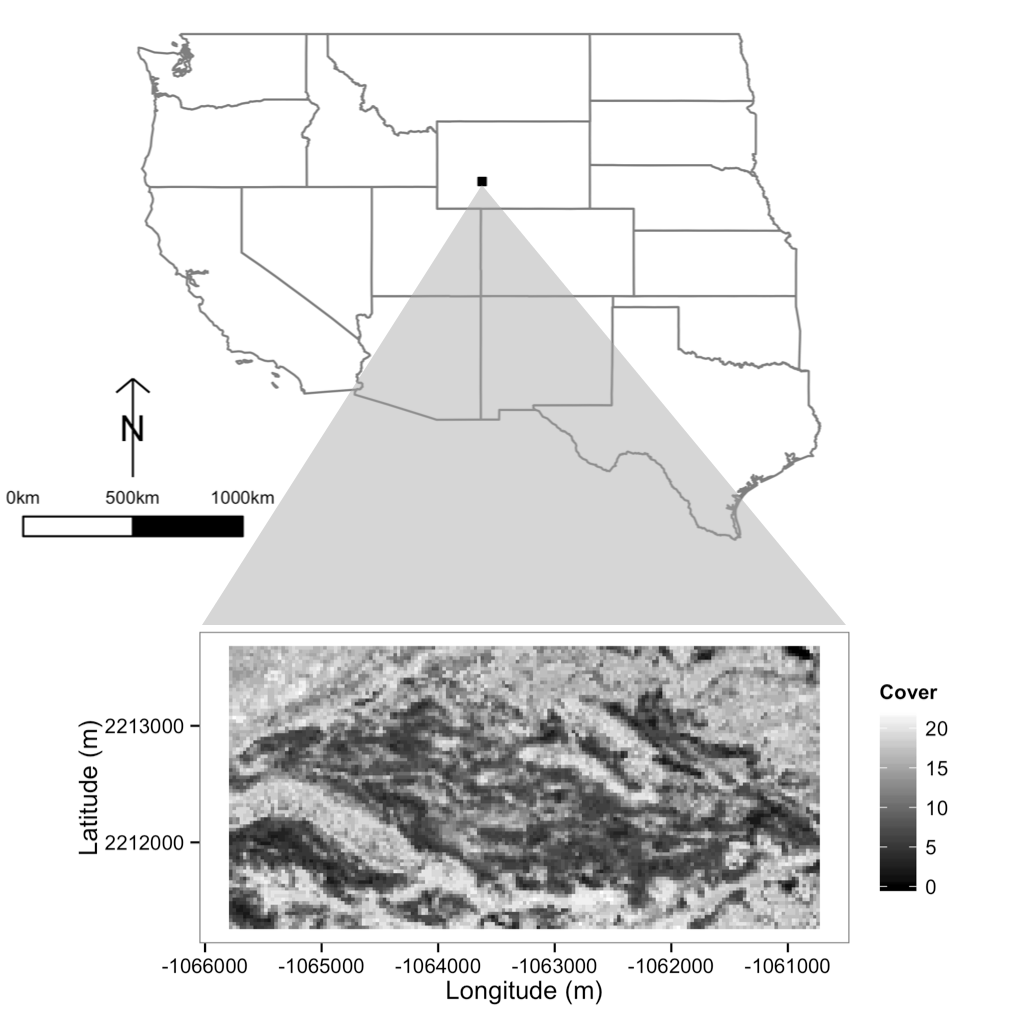
\includegraphics[height=6in]{../figures/studyarea_map.png}
  \caption{Location of the 5,070 $\times$ 2,430 meter kilometer study area in southwestern Wyoming (black rectangle) and a snapshot of the percent cover data in 1984 (detailed inset). Scale bar is relevant for US map only; refer to axes labels on the detailed inset of sagebrush percent cover for scale of the study area.}
\end{figure}

\newpage{}

\begin{figure}[!ht]
  \centering
      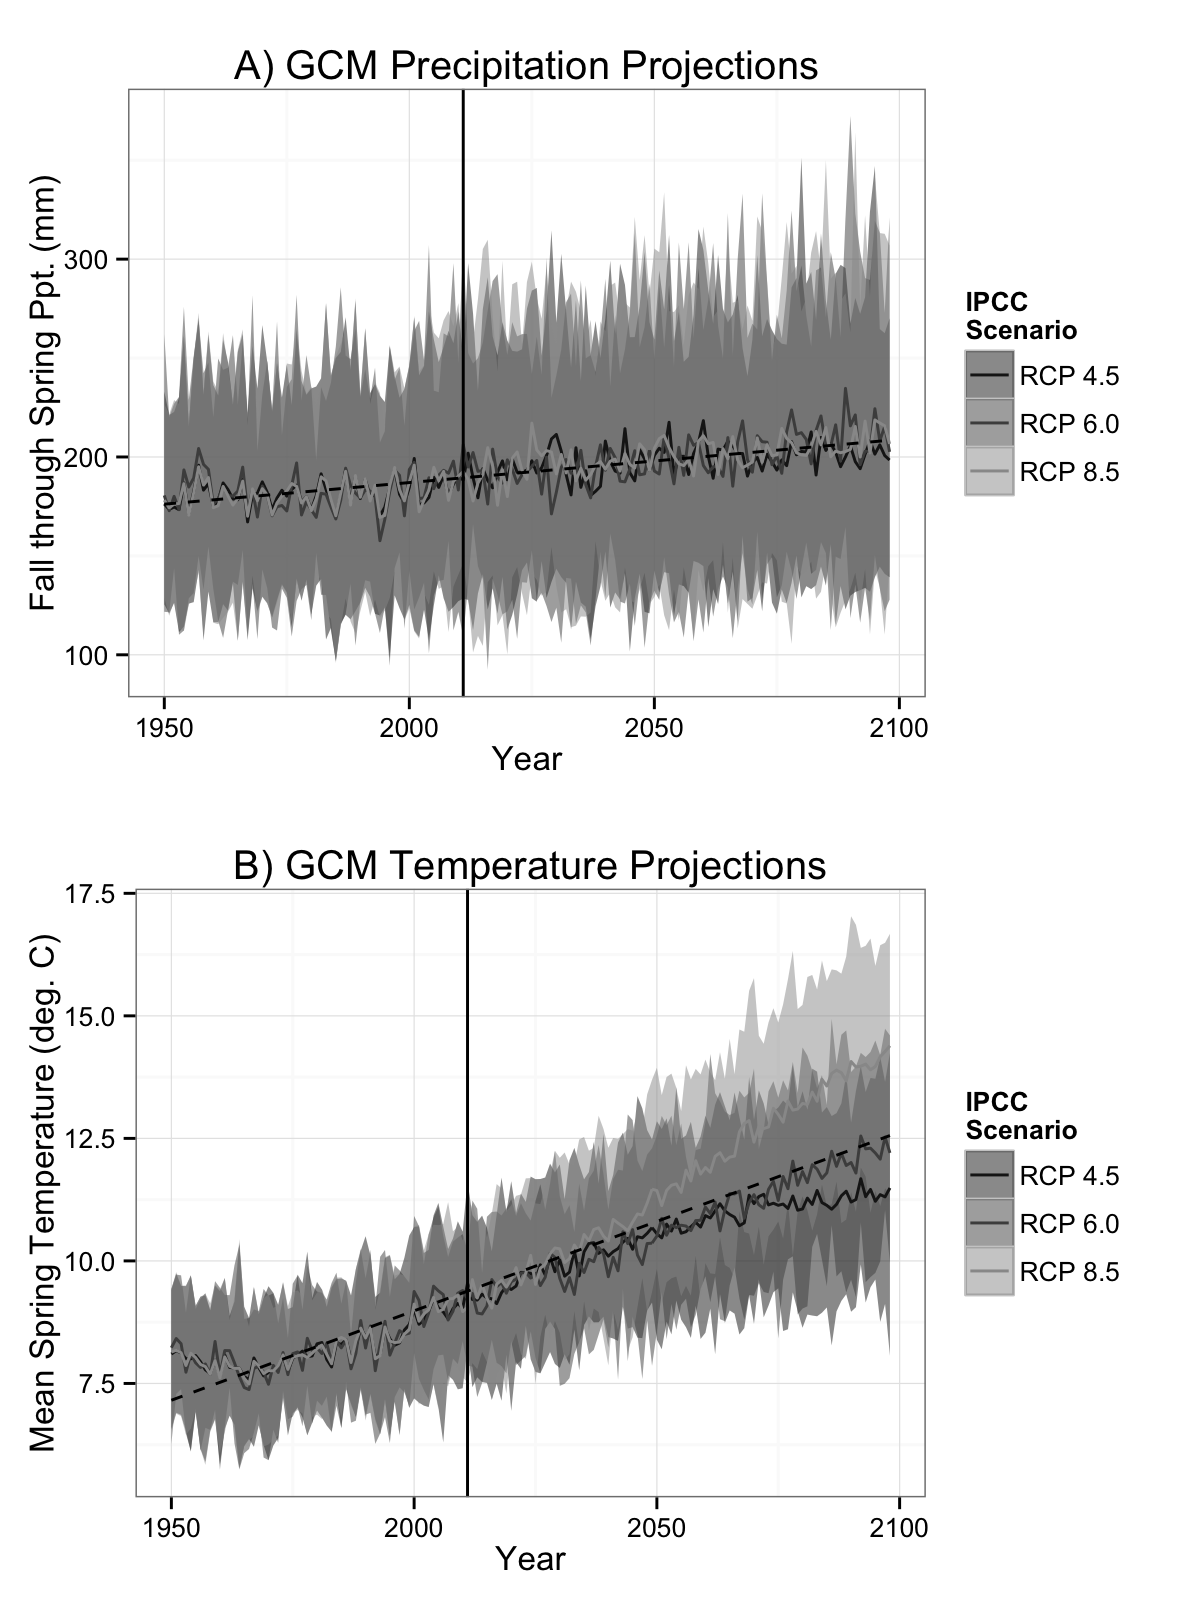
\includegraphics[width=4in]{../figures/weather_projections.png}
  \caption{GCM yearly weather hindcasts (before solid line at 2011) and projections (after solid line at 2011) for precipitation (A) and temperature (B) at our study area in southwestern Wyoming (see Fig. 1).}
\end{figure}

\newpage{}

\begin{figure}[!ht]
  \centering
      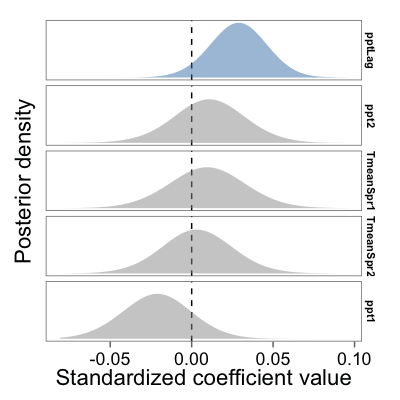
\includegraphics[width=4in]{../figures/post_climate_covariates.png}
  \caption{Posterior distributions of climate covariates. The x-axis is the standardized coefficient value because we fit the statistical model for sagebrush cover change (Eq. 7) using standardized covariate values. Only cumulative precipitation at time \emph{t-2} (pptLag) is important (shown in blue; 90\% CI does not overlap zero). Climate covariate codes: pptLag = water year precipitation in year \emph{t-2}; TmeanSpr1 = year \emph{t-1} average spring temperature; ppt2 = year \emph{t} fall through summer precipitation; TmeanSpr2 = year \emph{t} average spring temperature; ppt1 = year \emph{t-1} fall through summer precipitation.}
\end{figure}

\newpage{}

\begin{figure}[!ht]
  \centering
      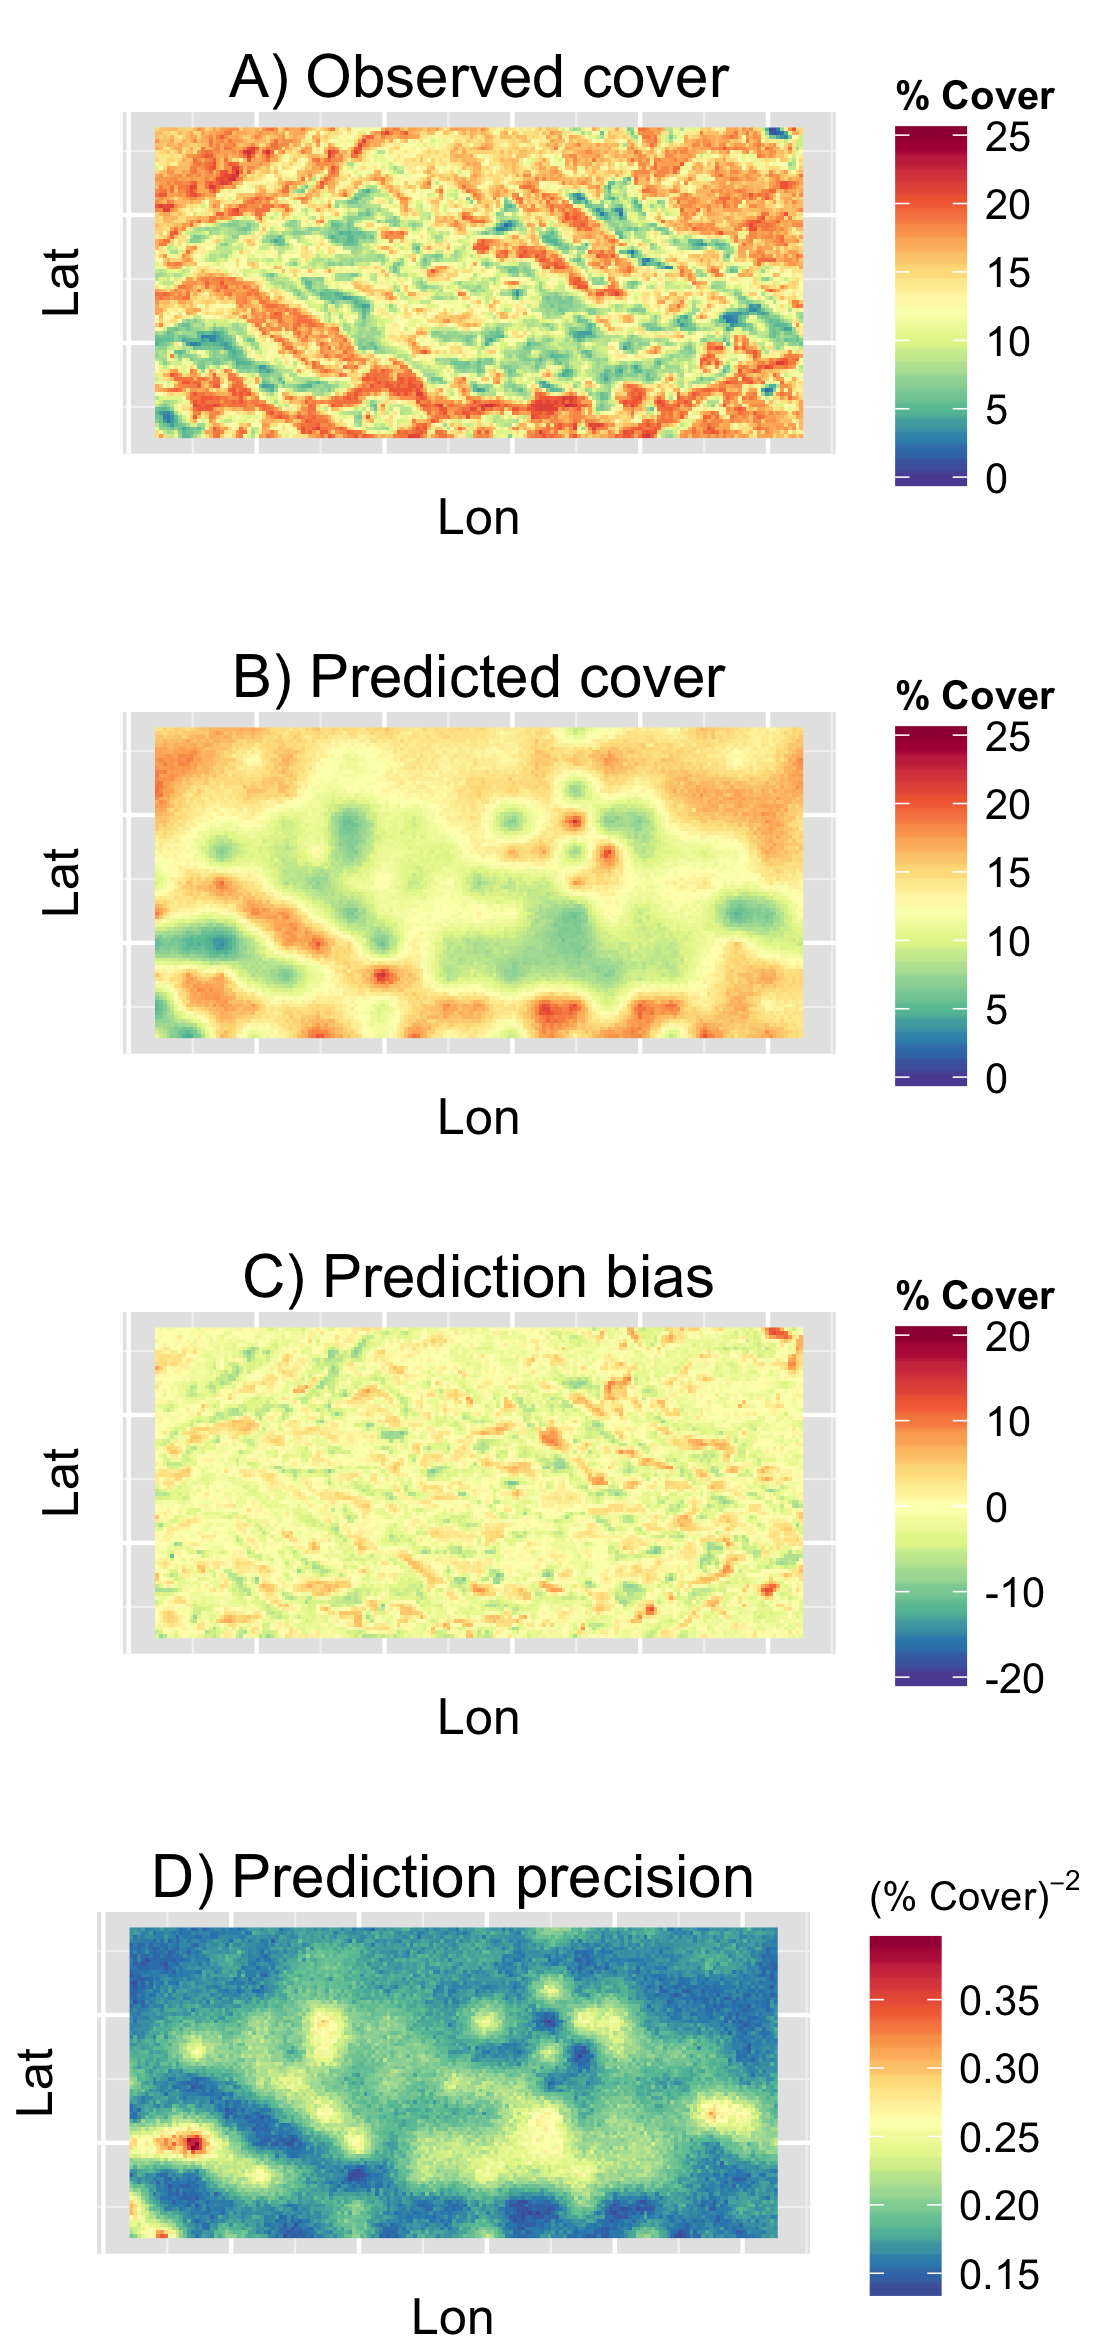
\includegraphics[height=6in]{../figures/obs_pred_spatial_subset.png}
  \caption{Observed and predicted (A, B) equilibrium percent cover of sagebrush, and prediction bias and precision (C, D) for the extent of our spatial area at 30-m resolution. Observed equilibrium sagebrush cover (A) is the temporal mean of each pixel from the 28 year time series. Prediction results are from simulations that use posteior mean parameter values. Precision in (D) represents the variability of each pixel over the course of the 2,000 iteration simulation. Axes definitions: Lat = latitude; Lon = longitude.}
\end{figure}

\newpage{}

\begin{figure}[!ht]
  \centering
      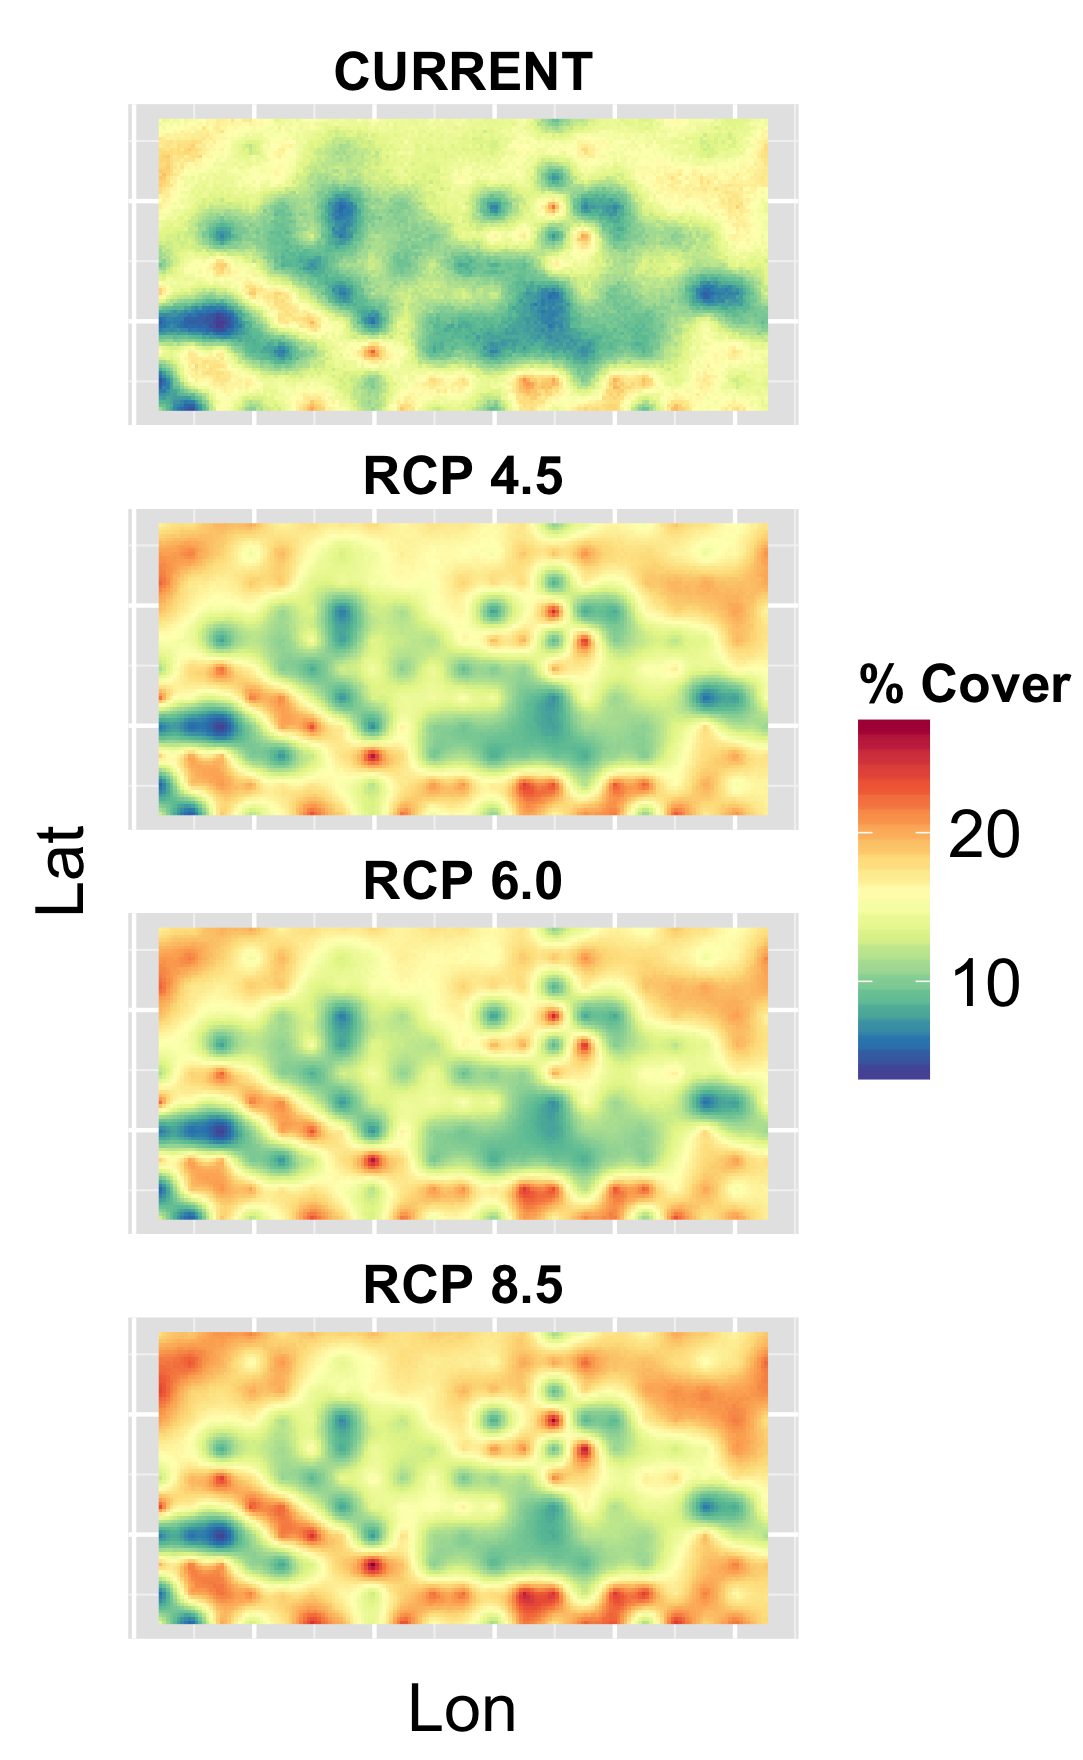
\includegraphics[height=6in]{../figures/clim_change_mean_spatial.png}
  \caption{Projected equilibrium cover under three IPCC climate change scenarios (RCP = Representative Concentration Pathways) for our study area in southwestern Wyoming. The top panel shows equilibrium cover based on simulations using observed climate. Subsequent panels show equilibrium cover based on perturbed climate for each RCP scenario. Forecasts are based on the projected climate changes in Table 1 applied to the observed climate time series used to fit the statistical model. We used posterior mean parameter estimates for all simulations. Color bar indicates percent cover of sagebrush in each 30x30 meter pixel. Axes definitions: Lat = latitude; Lon = longitude.}
\end{figure}

\newpage{}

\begin{figure}[!ht]
  \centering
      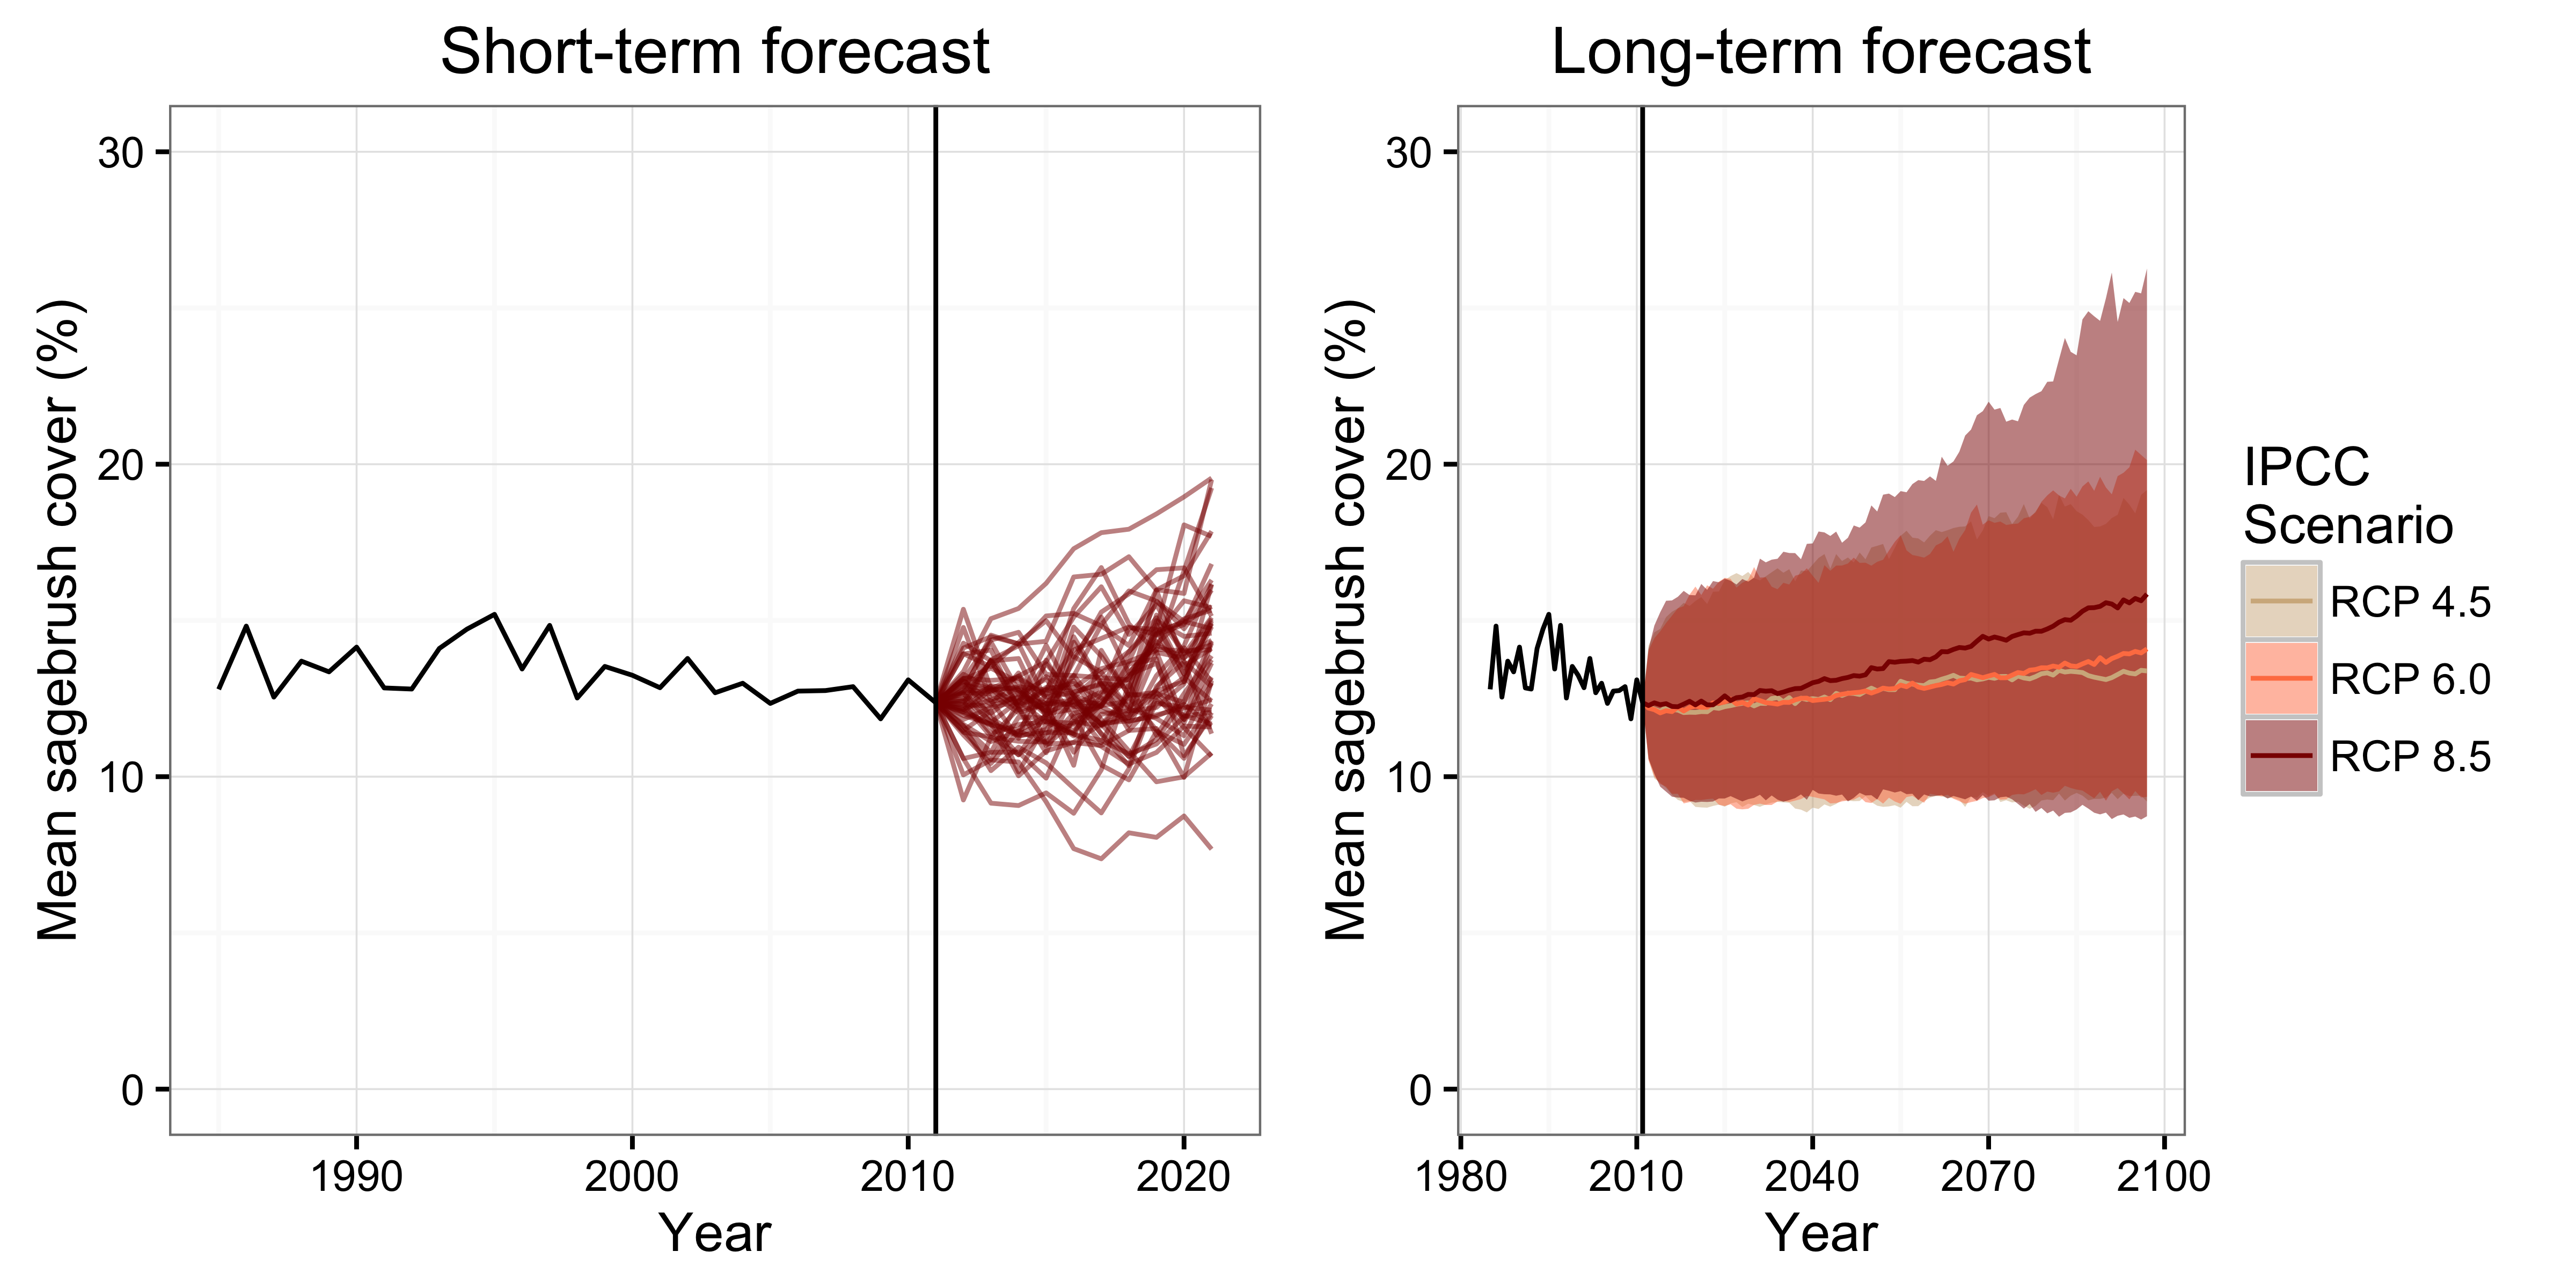
\includegraphics[width=3in]{../figures/figure6.png}
  \caption{Observed (black line before 2011) and forecasted (colored lines after 2011) sagebrush percent cover. Long-term forecasts (A) were made for three IPCC emissions scenarios (RCPs 4.5, 6.0, and 8.5) and are for the period of 2012 to 2098. Shaded regions show limits of the 5th and 95th quantiles for simulations conducted using 50 different sets of parameters from the MCMC output. Lines show mean trajectories. Uncertainty in forecasts arises from uncertainty in GCM projections, uncerainty around the ecological process, and uncertainty around parameter estimates. Before calculating the mean and quantiles for each year across parameter sets and GCMs, we averaged percent cover over the 13,689 pixels. \textcolor{blue}{Panel (B) shows an example short-term forecast (10 years) using the MIROC5 GCM projections under RCP 8.5. Each line shows a forecast from one parameter set.}}
\end{figure}

\newpage{}

\subsection*{References}\label{references}
\addcontentsline{toc}{subsection}{References}

Adler, P. B., H. J. Dalgleish, and S. P. Ellner. 2012. Forecasting plant
community impacts of climate variability and change: when do competitive
interactions matter? Journal of Ecology 100:478--487.

Apodaca, L. F. 2013. Assessing Growth Response to Climate Controls in a
Great Basin Artemisia Tridentata Plant Community. PhD thesis, University
of Nevada Las Vegas.

Arnett, E. B., and T. Z. Riley. 2015. Science, policy, and the fate of
the greater sage-grouse. Frontiers in Ecology and the Environment
13:235.

Baldeck, C. A., and G. P. Asner. 2014. Improving remote species
identification through efficient training data collection. Remote
Sensing 6:2682--2698.

Barry, R. P., and J. M. V. Hoef. 1996. Blackbox Kriging: Spatial
Prediction without Specifying Variogram Models.

Bradford, J. B., and W. K. Lauenroth. 2006. Controls over invasion of
Bromus tectorum: The importance of climate, soil, disturbance, and seed
availability. Journal of Vegetation Science 17:693--704.

Bradley, B. A. 2010. Assessing ecosystem threats from global and
regional change: hierarchical modeling of risk to sagebrush ecosystems
from climate change, land use and invasive species in Nevada, USA.
Ecography 33:198--208.

Bradshaw, G. A., and J. G. Borchers. 2000. Uncertainty as information:
Narrowing the science-policy gap. Ecology and Society 4.

Clark, J. S., D. M. Bell, M. H. Hersh, and L. Nichols. 2011. Climate
change vulnerability of forest biodiversity: Climate and competition
tracking of demographic rates. Global Change Biology 17:1834--1849.

Clark, J. S., S. R. Carpenter, M. Barber, S. Collins, A. Dobson, J. A.
Foley, D. M. Lodge, M. Pascual, R. Pielke, W. Pizer, C. Pringle, W. V.
Reid, K. A. Rose, O. Sala, W. H. Schlesinger, D. H. Wall, and D. Wear.
2001. Ecological forecasts: an emerging imperative. Science (New York,
N.Y.) 293:657--660.

Clark, J. S., A. E. Gelfand, C. W. Woodall, and K. Zhu. 2014. More than
the sum of the parts: Forest climate response from joint species
distribution models. Ecological Applications 24:990--999.

Colgan, M. S., and G. P. Asner. 2014. Coexistence and environmental
filtering of species-specific biomass in an African savanna. Ecology
95:1579--1590.

Conn, P. B., D. S. Johnson, J. M. V. Hoef, M. B. Hooten, J. M. London,
and P. L. Boveng. 2015. Using spatiotemporal statistical models to
estimate animal abundance and infer ecological dynamics from survey
counts. Ecological Monographs 85:235--252.

Dalgleish, H. J., D. N. Koons, M. B. Hooten, C. A. Moffet, and P. B.
Adler. 2011. Climate influences the demography of three dominant
sagebrush steppe plants. Ecology 92:75--85.

Debinski, D. M., H. Wickham, K. Kindscher, J. C. Caruthers, and M.
Germino. 2010. Montane meadow change during drought varies with
background hydrologic regime and plant functional group. Ecology
91:1672--81.

Ehrl{é}n, J., and W. F. Morris. 2015. Predicting changes in the
distribution and abundance of species under environmental change.
Ecology Letters 18:303--314.

Elith, J., and J. R. Leathwick. 2009. Species Distribution Models:
Ecological Explanation and Prediction Across Space and Time.

Ellner, S. P., and M. Rees. 2006. Integral projection models for species
with complex demography. The American naturalist 167:410--428.

Freckleton, R. P., W. J. Sutherland, A. R. Watkinson, and S. A.
Queenborough. 2011. Density-structured models for plant population
dynamics. American Naturalist 177:1--17.

Gelman, A., and J. Hill. 2009. Data analysis using regression and
multilevel/hierarchical models. Cambridge University Press, Cambridge.

Gelman, A., and D. B. Rubin. 1992. Inference from Iterative Simulation
Using Multiple Sequences. Statistical Science 7:457--472.

Gerber, B. D., W. L. Kendall, M. B. Hooten, J. A. Dubovsky, and R. C.
Drewien. 2015. Optimal population prediction of sandhill crane
recruitment based on climate-mediated habitat limitations. Journal of
Animal Ecology 84:1299--1310.

Germino, M. J., and K. Reinhardt. 2014. Desert shrub responses to
experimental modification of precipitation seasonality and soil depth:
Relationship to the two-layer hypothesis and ecohydrological niche.
Journal of Ecology 102:989--997.

Hare, J. a, M. a Alexander, M. J. Fogarty, E. H. Williams, and J. D.
Scott. 2010. Forecasting the dynamics of a coastal fishery species using
a coupled climate--population model. Ecological applications : a
publication of the Ecological Society of America 20:452--464.

Harte, J., S. R. Saleska, and C. Levy. 2015. Convergent ecosystem
responses to 23-year ambient and manipulated warming link advancing
snowmelt and shrub encroachment to transient and long-term climate-soil
carbon feedback. Global change biology 21:2349--56.

He, K. S., B. A. Bradley, A. F. Cord, D. Rocchini, M.-N. Tuanmu, S.
Schmidtlein, W. Turner, M. Wegmann, and N. Pettorelli. 2015. Will remote
sensing shape the next generation of species distribution models? Remote
Sensing in Ecology and Conservation 1:4--18.

Higdon, D. 1998. A process-convolution approach to modelling
temperatures in the North Atlantic Ocean. Environmental and Ecological
Statistics 5:173--190.

Higdon, D. M. 2002. Space and space-time modeling using process
convolutions. Pages 37--56 \emph{in} C. Anderson, V. Barnett, P.
Chatwin, and A. El-Shaarawi, editors. Quantitative methods for current
environmental issues. Springer, London.

Hobbs, N. T., and M. B. Hooten. 2015. Bayesian Models: A Statistical
Primer for Ecologists. Princeton University Press, Princeton.

Homer, C. G., C. L. Aldridge, D. K. Meyer, and S. J. Schell. 2012.
Multi-scale remote sensing sagebrush characterization with regression
trees over Wyoming, USA: Laying a foundation for monitoring.
International Journal of Applied Earth Observation and Geoinformation
14:233--244.

Homer, C. G., G. Xian, C. L. Aldridge, D. K. Meyer, T. R. Loveland, and
M. S. O'Donnell. 2015. Forecasting sagebrush ecosystem components and
greater sage-grouse habitat for 2050: Learning from past climate
patterns and Landsat imagery to predict the future. Ecological
Indicators 55:131--145.

Hooten, M. B., and N. T. Hobbs. 2015. A guide to Bayesian model
selection for ecologists. Ecological Monographs 85:3--28.

Hooten, M. B., and C. K. Wikle. 2007. Shifts in the spatio-temporal
growth dynamics of shortleaf pine. Environmental and Ecological
Statistics 14:207--227.

Hooten, M. B., D. R. Larsen, and C. K. Wikle. 2003. Predicting the
spatial distribution of ground flora on large domains using a
hierarchical Bayesian model. Landscape Ecology 18:487--502.

Kuchler, A. 1964. Potential Natural Vegetation of the Conterminous
United States. American Geographical Society, Special Publication No.
36.

Latimer, A. M., S. Banerjee, H. Sang, E. S. Mosher, and J. A. Silander.
2009. Hierarchical models facilitate spatial analysis of large data
sets: A case study on invasive plant species in the northeastern United
States. Ecology Letters 12:144--154.

Luo, Y., K. Ogle, C. Tucker, S. Fei, C. Gao, S. LaDeau, J. S. Clark, and
D. S. Schimel. 2011. Ecological forecasting and data assimilation in a
data-rich era. Ecological Applications 21:1429--1442.

Maiorano, L., R. Cheddadi, N. E. Zimmermann, L. Pellissier, B.
Petitpierre, J. Pottier, H. Laborde, B. I. Hurdu, P. B. Pearman, A.
Psomas, J. S. Singarayer, O. Broennimann, P. Vittoz, A. Dubuis, M. E.
Edwards, H. A. Binney, and A. Guisan. 2013. Building the niche through
time: using 13,000 years of data to predict the effects of climate
change on three tree species in Europe. Global Ecology and Biogeography
22:302--317.

Merow, C., A. M. Latimer, A. M. Wilson, S. M. McMahon, A. G. Rebelo, and
J. A. Silander. 2014. On using integral projection models to generate
demographically driven predictions of species' distributions:
development and validation using sparse data. Ecography 37:1167--1183.

Miglia, K., E. Mcarthur, W. Moore, H. Wang, J. Graham, and D. Freeman.
2005. Nine-year reciprocal transplant experiment in the gardens of the
basin and mountain big sagebrush (Artemisia tridentata: Asteraceae)
hybrid zone of Salt Creek Canyon: the importance of multiple-year
tracking of fitness Title. Biological Journal of the Linnean
Society:213--225.

Neilson, R., J. Lenihan, D. Bachelet, and R. Drapek. 2005. Climate
change implications for sagebrush ecosystems. Page 145 \emph{in} North
american wildlife and natural resources conference.

Pechanec, J., G. Pickford, and G. Stewart. 1937. Effects of the 1934
Drought on Native Vegetation of the Upper Snake River Plans, Idaho.
Ecology:490--505.

Perfors, T., J. Harte, and S. E. Alter. 2003. Enhanced growth of
sagebrush (Artemisia tridentata) in response to manipulated ecosystem
warming. Global Change Biology 9:736--742.

Petchey, O. L., M. Pontarp, T. M. Massie, S. K{é}fi, A. Ozgul, M.
Weilenmann, G. M. Palamara, F. Altermatt, B. Matthews, J. M. Levine, D.
Z. Childs, B. J. McGill, M. E. Schaepman, B. Schmid, P. Spaak, A. P.
Beckerman, F. Pennekamp, and I. S. Pearse. 2015. The ecological forecast
horizon, and examples of its uses and determinants. Ecology Letters
18:597--611.

Poore, R. E., C. A. Lamanna, J. J. Ebersole, and B. J. Enquist. 2009.
Controls on Radial Growth of Mountain Big Sagebrush and Implications for
Climate Change. Western North American Naturalist 69:556--562.

Queenborough, S. A., K. M. Burnet, W. J. Sutherland, A. R. Watkinson,
and R. P. Freckleton. 2011. From meso- to macroscale population
dynamics: A new density-structured approach. Methods in Ecology and
Evolution 2:289--302.

R Core Team. 2013. R: A language and environment for statistical
computing.

Rees, M., and S. P. Ellner. 2009. Integral projection models for
populations in temporally varying environments. Ecological Monographs
79:575--594.

Roberts, D. R., and A. Hamann. 2012. Predicting potential climate change
impacts with bioclimate envelope models: A palaeoecological perspective.
Global Ecology and Biogeography 21:121--133.

Ross, B. E., M. B. Hooten, J.-M. DeVink, and D. N. Koons. 2015. Combined
effects of climate, predation, and density dependence on Greater and
Lesser Scaup population dynamics. Ecological Applications 25:1606--1617.

Running, S. W., R. R. Nemani, F. A. Heinsch, M. Zhao, M. Reeves, and H.
Hashimoto. 2004. A Continuous Satellite-Derived Measure of Global
Terrestrial Primary Production. BioScience 54:547.

Rupp, D. E., J. T. Abatzoglou, K. C. Hegewisch, and P. W. Mote. 2013.
Evaluation of CMIP5 20th century climate simulations for the Pacific
Northwest US. Journal of Geophysical Research 118:1--23.

Salguero-G{ó}mez, R., O. R. Jones, C. R. Archer, Y. M. Buckley, J.
Che-Castaldo, H. Caswell, D. Hodgson, A. Scheuerlein, D. A. Conde, E.
Brinks, H. de Buhr, C. Farack, F. Gottschalk, A. Hartmann, A. Henning,
G. Hoppe, G. R{ö}mer, J. Runge, T. Ruoff, J. Wille, S. Zeh, R. Davison,
D. Vieregg, A. Baudisch, R. Altwegg, F. Colchero, M. Dong, H. de Kroon,
J.-D. Lebreton, C. J. E. Metcalf, M. M. Neel, I. M. Parker, T. Takada,
T. Valverde, L. A. V{é}lez-Espino, G. M. Wardle, M. Franco, and J. W.
Vaupel. 2015. The compadrePlant Matrix Database: an open online
repository for plant demography. Journal of Ecology 103:202--218.

Schlaepfer, D. R., W. K. Lauenroth, and J. B. Bradford. 2011.
Ecohydrological niche of sagebrush ecosystems. Ecohydrology:n/a--n/a.

Schlaepfer, D. R., W. K. Lauenroth, and J. B. Bradford. 2014a. Modeling
regeneration responses of big sagebrush (Artemisia tridentata) to
abiotic conditions. Ecological Modelling 286:66--77.

Schlaepfer, D., W. K. Lauenroth, and J. B. Bradford. 2012. Effects of
ecohydrological variables on current and future ranges, local
suitability patterns, and model accuracy in big sagebrush. Ecography
5:453--466.

Schlaepfer, D., W. K. Lauenroth, and J. B. Bradford. 2014b. Natural
Regeneration Processes in Big Sagebrush (Artemisia tridentata).
Rangeland Ecology \& Management 67:344--357.

Schurr, F. M., J. Pagel, J. S. Cabral, J. Groeneveld, O. Bykova, R. B.
O'Hara, F. Hartig, W. D. Kissling, H. P. Linder, G. F. Midgley, B.
Schr{ö}der, A. Singer, and N. E. Zimmermann. 2012. How to understand
species' niches and range dynamics: A demographic research agenda for
biogeography. Journal of Biogeography 39:2146--2162.

Shafer, S. L., P. J. Bartlein, and R. S. Thompson. 2001. Potential
changes in the distributions of western North America tree and shrub
taxa under future climate scenarios. Ecosystems 4:200--215.

Shriver, R. K. 2015. Quantifying how short-term environmental variation
leads to long-term demographic responses to climate change. Journal of
Ecology:n/a--n/a.

Stan Development Team. 2014a. Stan: A C++ Library for Probability and
Sampling, Version 2.5.0.

Stan Development Team. 2014b. Rstan: the R interface to Stan, Version
2.5.0.

Still, S., and B. Richardson. 2015. Projections of Contemporary and
Future Climate Niche for Wyoming Big Sagebrush (Artemisia tridentata
subsp. wyomingensis): A Guide for Restoration. Natural Areas Journal
35:30--43.

Vanderwel, M. C., V. S. Lyutsarev, and D. W. Purves. 2013.
Climate-related variation in mortality and recruitment determine
regional forest-type distributions. Global Ecology and Biogeography
22:1192--1203.

Wikle, C. K. 2010. Low-rank representations for spatial processes. Pages
89--106 \emph{in} A. Gelfand, P. Diggle, M. Fuentes, and P. Guttopr,
editors. Handbook of spatial statistics. Chapman; Hill, Upper Saddle
River, New Jersey, USA.

Xian, G., C. G. Homer, and C. L. Aldridge. 2012. Effects of Land Cover
and Regional Climate Variations on Long-Term Spatiotemporal Changes in
Sagebrush Ecosystems. GIScience \& Remote Sensing 49:378--396.

\end{document}
